\documentclass[a4paper, 11pt]{article}
\usepackage{comment} % enables the use of multi-line comments (\ifx \fi) 
\usepackage{lipsum} %This package just generates Lorem Ipsum filler text. 
\usepackage{fullpage} % changes the margin
\usepackage{graphicx}
\usepackage{caption}
\usepackage{subcaption}

\begin{document}
%Header-Make sure you update this information!!!!
\noindent
\large\textbf{Machine Learning Project report} \hfill \textbf{Jiyan Jonsdotter} \\
\normalsize ML \hfill \textbf{Massimo Innocentini} \\
Dr. Norman Hendrich \\
TA: Philipp Ruppel \hfill Due Date: 30/06/2018

\section*{Introduction}
The dataset that we decided to analyse is from the Forest Cover Type competition. The goal of the competition is to predict the type of forest, given a set of features, hence It is a multi-class classification problem. Kaggle provides a training set of data with the forest cover type, in total there are 15120 observations, and a test data set with only the observed features with 565892 samples. There are 7 type of forest cover used in the competition, each assigned an integer number: 

\begin{enumerate}
  \item \texttt{Spruce/Fir}
  \item \texttt{Lodgepole Pine}
  \item \texttt{Ponderos Pine}
  \item \texttt{Cottonwood/Willow}
  \item \texttt{Aspen}
  \item \texttt{Douglas-fir}
  \item \texttt{Krummholz}
\end{enumerate}

There are 13 type of features which describe a 30m x 30m area in each sample, the features are:

\begin{itemize}
  \item \texttt{Elevation}: 
  \item \texttt{Aspect}: 
  \item \texttt{Slope}: 
  \item \texttt{Horizontal\_Distance\_To\_Hydrology}: 
  \item \texttt{Vertical\_Distance\_To\_Hydrology}: 
  \item \texttt{Horizontal\_Distance\_to\_Roadways}: 
  \item \texttt{Hillshade\_9am}: 
  \item \texttt{Hillshade\_Noon}:
  \item \texttt{Hillshade\_3pm}:
  \item \texttt{Horizontal\_Distance\_To\_Fire\_Points}: 
  \item \texttt{Wilderness\_Area}: 
  \item \texttt{Soil\_Type}: 
  \item \texttt{Cover\_Type} :
\end{itemize} 

Few of those terms are clear like elevation, however there some of them need further explanation. The \texttt{Slope} and \texttt{Aspect} identify respectively the land inclination and the direction of the inclination in degrees. The hydrology distance reports the distance from the closest water source. The hill shade is a grayscale representation value of the illumination of the surface, which takes into account the position of the sun at different times. The values returned range from 0 to 255.

\texttt{Wilderness area} is divided into 4 groups: Rawah , Neota, Comanche Peak and Cache la Poudre. For simplicity in the dataset each is assigned an integer number. As the name suggests wilderness area are reservations which are untouched by humans in order to prevent natural conditions and wildlife. Finally the \texttt{Soil type} is also divided into subgroups, the data identifies 40 of them. Every feature is of integer type.

\section*{Data Analysis}
The initial analysis performed on the data showed that few of the feature resemble a normal distribution, like \texttt{Hillshade\_3pm} or the \texttt{Slope} distribution, plus the variance for those features is also closer to 1. After computing the mean of each column we noticed that there is definitely an imbalance among the values of the columns. For instance elevation seems to be measured in meters, while the slope if the land is measured in degrees, in this case one has a mean of 2700 while the other of 16 accordingly. We believe this will cause bias during the training phase and the data should be normalised.

Another imbalance noticed in the features is that even though there are 40 types of soil type, type 10 occurrence is way higher than the others, moreover there seems to be redundant information while plotting the forest cover type with the type of soil. The redundancy was noticed with the wilderness areas too. Finally some feature like \texttt{Hillshade\_Noon} seems to be constant among all the samples hence not really representing anything useful.

\section*{Interesting Features}
We tried plotting most features against the forest cover type in order to view if there was correlation. There were few that showed potential influence on the resulting forest as can be seen from plots Fig \ref{elev}, \ref{fire}, \ref{road}, \ref{hydro}. The plot in Fig \ref{hydro} shows how the forest type changes based on the distance from water. The plot merge both the vertical and horizontal distance from water and each colour in the plot indicated a kind of forest cover. The idea was taken from the Kernel of skillsmuggler \cite{skill}, where the author plot both distances from the water but uses elevation as a colour. From the plot It does look like it can be an interesting feature.

\begin{figure}[htb]
\centering
\begin{minipage}{.5\textwidth}
  \centering
  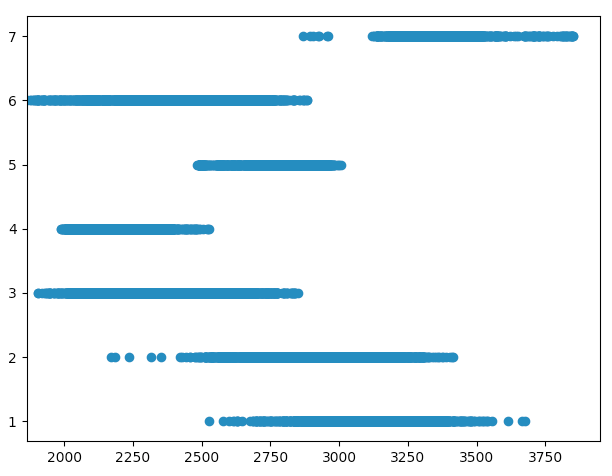
\includegraphics[width=\textwidth]{img/elevation}
  \captionof{figure}{Elevation / forest cover type}
  \label{elev}
\end{minipage}%
\begin{minipage}{.5\textwidth}
  \centering
  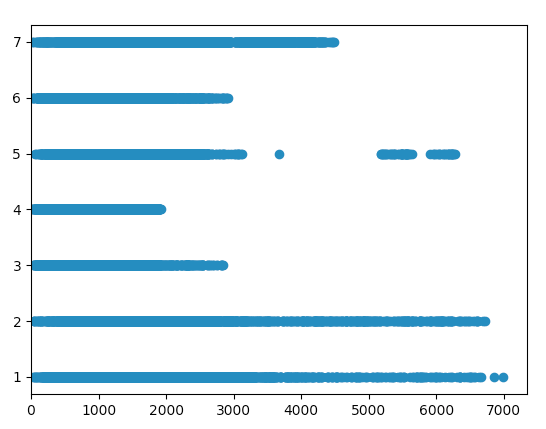
\includegraphics[width=\textwidth]{img/distance_to_fire_points}
  \captionof{figure}{Fire points distance / forest cover type}
  \label{fire}
\end{minipage}
\end{figure}

\begin{figure}[htb]
\centering
\begin{minipage}{.5\textwidth}
  \centering
  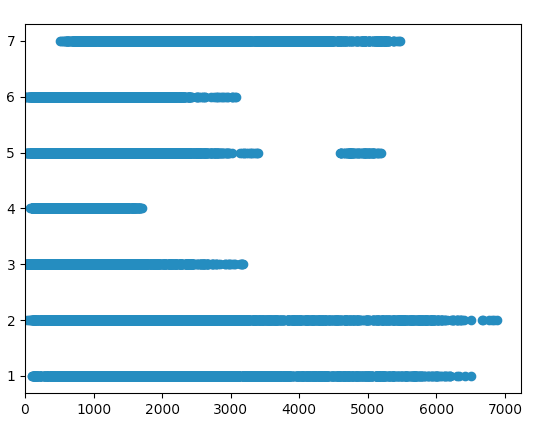
\includegraphics[width=\textwidth]{img/distance_to_roads}
  \captionof{figure}{Roads distance / forest cover type}
  \label{road}
\end{minipage}%
\begin{minipage}{.5\textwidth}
  \centering
  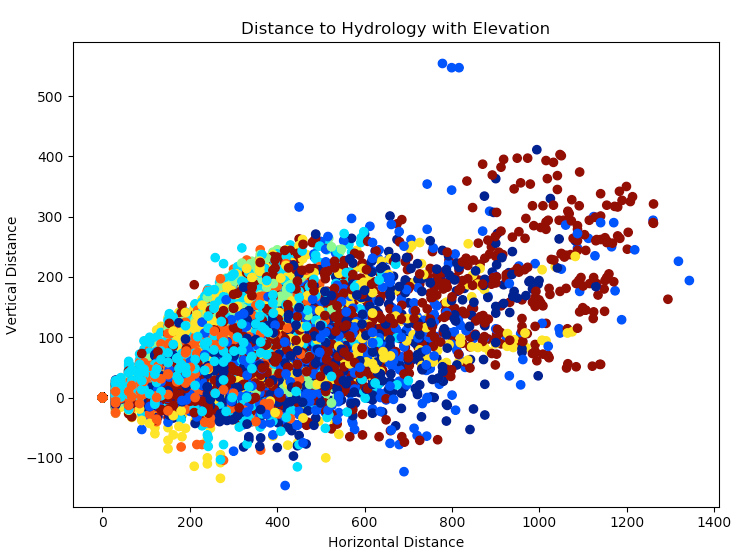
\includegraphics[width=1.05\textwidth]{img/hydrology_distance}
  \captionof{figure}{Water distance / forest cover type}
  \label{hydro}
\end{minipage}
\end{figure}

The other two features which seemed interested during the exploration of the data, were the soil type and maybe the wilderness area. In particular during the analysis we noticed that a certain kind of forest type was linked to few soil types, like Fig \ref{soil1} and \ref{soil2} shows. However It is necessary to mention as said before that we had redundancy information and similar soil type were also found with the same forest cover type. 

\begin{figure}[htb]
\centering
\begin{minipage}{.5\textwidth}
  \centering
  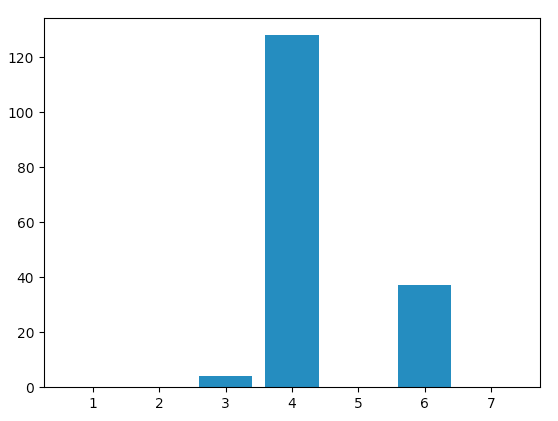
\includegraphics[width=1.01\textwidth]{img/soil_type_14}
  \captionof{figure}{Soil type 14 / forest cover type}
  \label{soil1}
\end{minipage}%
\begin{minipage}{.5\textwidth}
  \centering
  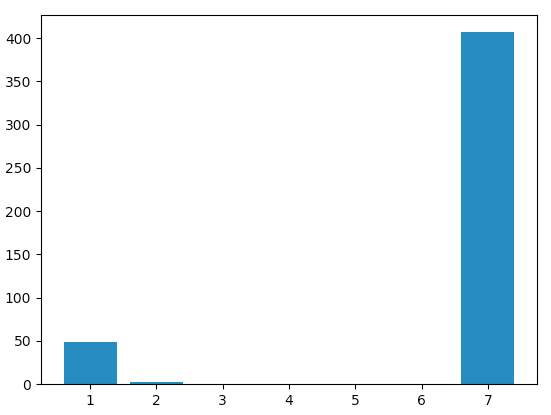
\includegraphics[width=1\textwidth]{img/soil_type_40}
  \captionof{figure}{Soil type 40 / forest cover type}
  \label{soil2}
\end{minipage}
\end{figure}

\section*{Data Processing Findings}
We tried to run a simple clustering algorithm using kmeans with k= [3,4,5,6,7,8,9,10] however the result were not promising, the silhouette score mean was around 0. That means that the clusters found were not actually indicating representative features.

Moreover we applied PCA just to check the results are shown in Fig \ref{pca}, we followed the sklearn example to plot the result according to the difference classes we had in our dataset. The result of the components are also not helpful since there is not a single component which held a high variance. Which means there does not seems to be a subgroup of feature which overwhelm the others. Anyway the dataset provided does not have too many features so the the training of the model should still be efficient. The only extra feature which should be reduce are the soil types and wilderness area since now they are split in multiple columns. One way is to either use a range to split to merge them or at least compress them into a single column like \cite{skill} does. The former seems to be more plausible and the least likely to lose important features.

\begin{figure}[htb]
\centering
  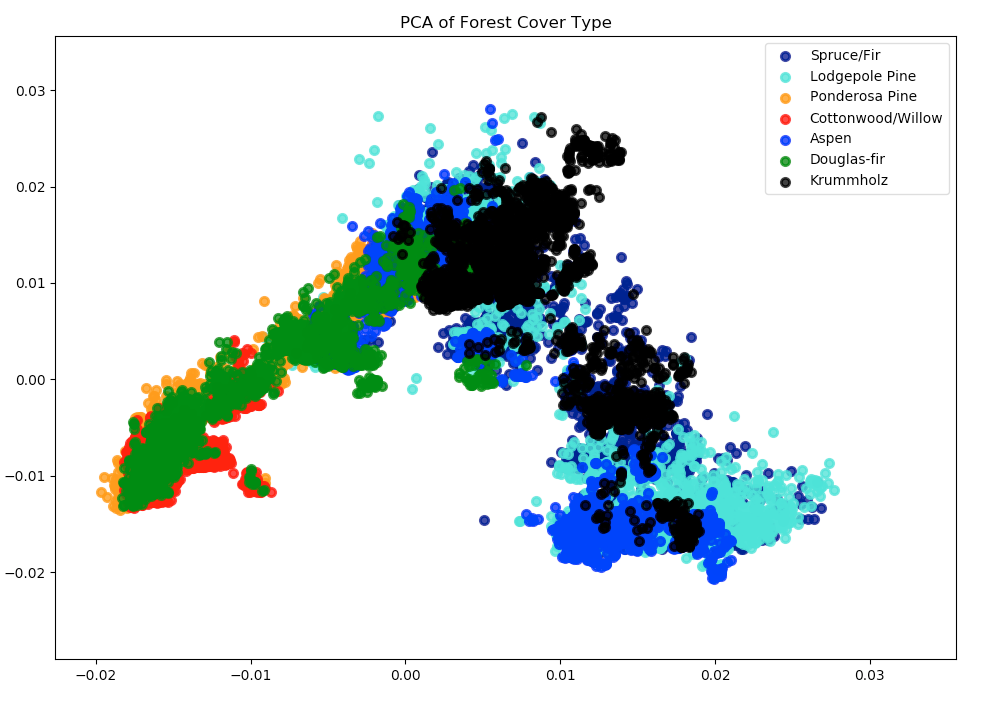
\includegraphics[width=0.8\textwidth]{img/pca}
  \captionof{figure}{PCA applied on the dataset}
  \label{pca}
\end{figure}

Finally an interesting feature of the data is the wilderness area, which at the moment we don't know how to consider with the respect to the future model. As we described in the introduction, those areas are uncontaminated by human, hence in a way their different from areas not protected because there humans can affect the forest in addition natural characteristics of the land. For instance as you can see from Fig \ref{wild}, when the zone is considered a wilderness area of type 4 when there is a forest cover of either type 3 or 4 with strong probability given the occurrences.

\begin{figure}[htb]
\centering
  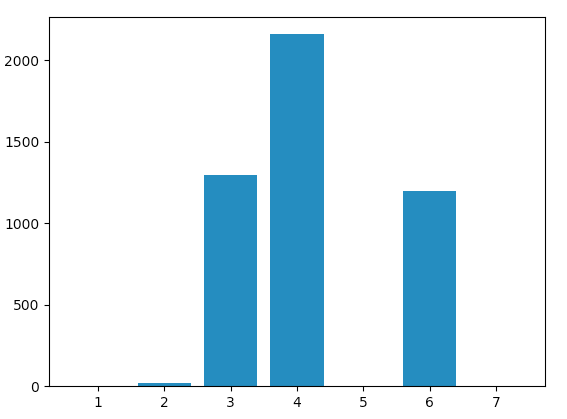
\includegraphics[width=0.8\textwidth]{img/wild_area_4}
  \captionof{figure}{Wilderness area 4 in respect to forest cover type.}
  \label{wild}
\end{figure}

\section*{Conclusion}
In conclusion we believe that the features which will play an important role are the distances from: fire, water and roads, the elevation of the area will also quite likely have an impact on the type of forest to be found as we have seen from Fig \ref{elev}. The other features seems to be less representative, except for the soil type which we will need to asses during training. Since this is a multi-class classification problem, we will probably try to use the basic K-nearest-neighbors at the beginning to see the results, then move on to SVM and if we have enough time, implement a deep neural network which should perform better given the nature of the problem.

\begin{thebibliography}{9}
\bibitem{skill} skillsmuggler. https://www.kaggle.com/skillsmuggler/eda-and-dimension-reduction
\bibitem{sklearn}Scikit-learn tutorials. http://scikit-learn.org/stable/tutorial/index.html
\end{thebibliography}

\end{document}